\subsection{Redigering af brugeroplysninger}
Brugeren skal ud fra app'ens hovedmenu have mulighed for at redigere private samt sygdomsspecifikke oplysninger. Dette er med henblik på, at brugeren selv skal kunne ændre sin adgangskode samt sin kategorisering, hvis deres helbred forværres. Af \autoref{fig:Redigerbrugeroplysninger} er aktivitetsdiagrammet for redigering af brugeroplysninger illustreret. 

\begin{figure} [H]
\centering
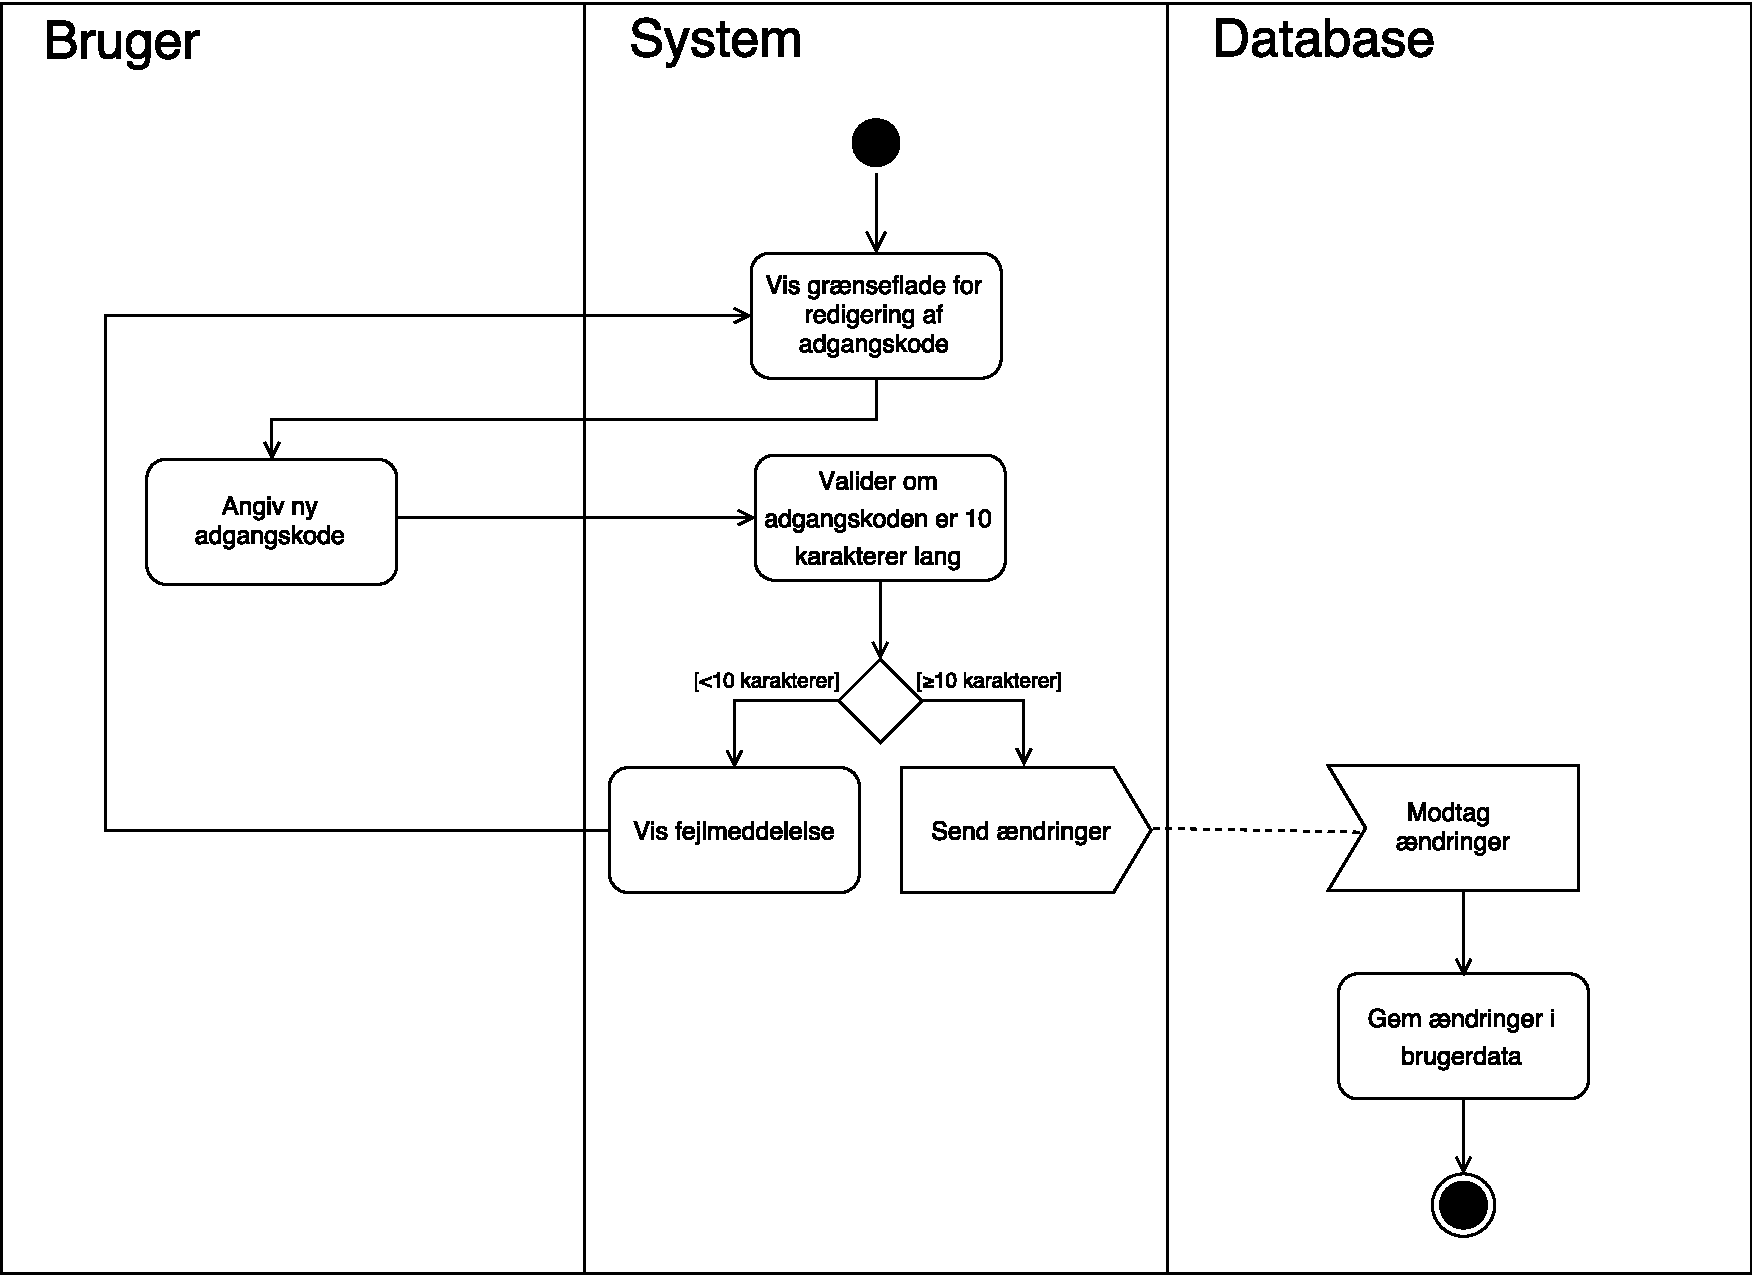
\includegraphics[width=0.9\textwidth]{figures/aktivitetsdiagram/Redigerbrugeroplysninger}
\caption{Aktivitetsdiagram for redigering af brugeroplysninger.}
\label{fig:Redigerbrugeroplysninger}
\end{figure}

Det skal både være muligt at ændre sin adgangskode samt kategoriseringen, som blev defineret første gang brugeren loggede ind på app'en. Da brugeren ved registrering får tildelt en tilfældig adgangskode, jf. \autoref{sec:registrering}, skal det være muligt at ændre denne til en personlig adgangskode. For at kunne foretage en ændring af adgangskoden, skal den nye adgangskode som minimum være seks karakterer lang. Hvis dette ikke opfyldes sendes en fejlmeddelse tilbage til brugeren, hvortil en ny adgangskode skal indtastes. 
I tilfælde af, at brugerens tilstand ændres er det ligeledes muligt at redigere denne. I \autoref{sec:kategorisering} beskrives aktivtetsdiagrammet for kategoriseringen af KOL yderligere. 
Ved korrekt redigering af brugeroplysninger sendes ændringerne til databasen, hvorefter de gemmes.